\section{Cylinder partition functions and contour sectors}
\label{sec:02-cylinder}

Our first task is to express the positive cylinder observable as a
finite sum to which asymptotic analysis can be applied. We prove two
exact representations: a sum over three labels at each site, and an
integral over finitely many contour sectors. The normalization is part
of each identity. We then estimate that normalization on the balanced
physical cylinder. The construction begins with the strip estimate needed to control
paths in a fixed-width periodic slab. The positive length--nest
comparison will be proved with its applications in
Section~\ref{sec:05-nesting}.

We use the honeycomb lattice dual to the equilateral triangular lattice
of side length one. A port is the midpoint of a tile edge. A path between
ports visits each honeycomb vertex at most once, includes its endpoint
half-edges, and has weight $\rho^{n(\gamma)}$, where $n(\gamma)$ counts
visited vertices. A polygon of length $r$ has $r$ vertices. Put
\[
 \lambda=\frac\pi8,\qquad
 d=\cos(2\lambda)=\frac1{\sqrt2},\qquad c=\cos(3\lambda),\qquad
 \rho=\frac1{\sqrt{2+\sqrt2}}.
\]
For the strip of $H$ triangular bands, let $\mathcal A_H$ be the mass
of paths from one fixed bottom port to the other bottom ports and let
$\mathcal B_H$ be their mass to the top boundary. We use the following
results from \cite[Theorem 1.1 and Lemmas 2.1, 2.3]{StripCompanion}:
\begin{equation}\label{eq:E-strip-input}
 c\mathcal A_H+\mathcal B_H=1,\qquad
 0<\mathcal B_H\asymp H^{-1/4},\qquad
 \mathcal B_H\text{ is nonincreasing in }H.
\end{equation}
The same source proves exponential decay of a one-defect transfer at
each fixed height, and boundedness of the corresponding vacuum
half-state. Here a defect means one strand attached to a specified
source and continuing to the current cut. We will name each use of
these finite-height facts.

\subsection{Strip input and the critical walk bound}

The critical activity is the reciprocal of the connective constant,
as proved by Duminil-Copin and Smirnov~\cite{DCS2012}. For later use
we give the short deduction from the strip estimates; it also supplies
a subexponential bound without a limit interchange.

\begin{proposition}[Critical weight]\label{prop:02-critical}
If $c_n$ is the number of $n$-edge self-avoiding walks from a specified
honeycomb vertex and $\mu=\lim_{n\to\infty}c_n^{1/n}$, then
$\rho=\mu^{-1}$. Moreover, $c_n\rho^n=\exp(o(n))$ as an upper bound.
\end{proposition}
\begin{proof}
We use the bridge-decomposition method of Hammersley and
Welsh~\cite{HammersleyWelsh1962}; see also
Madras and Slade~\cite{MadrasSlade1993} and
Duminil-Copin and Hammond~\cite[Proposition~2.1]{DuminilCopinHammond2013}.
We give the decomposition with the present honeycomb endpoint conventions,
using the positive strip bound to control each weak bridge.

Submultiplicativity gives existence of $\mu$. Split a walk at a vertex
of minimum height, choosing the first such vertex in a fixed traversal
order when necessary. Its two tails start at that vertex and stay above
its height. Translate this vertex to one of two fixed representatives,
according to its triangular-band type. Recording the two tails and the
split time recovers the original walk, because its original root is fixed.

Decompose each nonempty tail by stopping at its last global maximum,
then at the last minimum of the remainder, and continuing alternately.
Every piece is a weak bridge: all its vertices lie between the heights
of its endpoints. There are no horizontal edges. Its positive spans,
measured in thirds of a triangular band, are integers, are nonincreasing,
and are strictly decreasing after a possible equality of the first two.
Their sum is at most $2n$. Consequently there are $O(\sqrt n)$ pieces
and at most $\exp(O(\sqrt n\log(n+1)))$ possible span lists, even after
recording the split time and the two initial types.

For a fixed initial vertex and a specified directed span, the total
$\rho^{\#\text{edges}}$-weight of weak bridges is bounded by an absolute
constant. To obtain this from the strip bound $\mathcal B_H\le1$,
choose horizontal band boundaries immediately beyond the two endpoint
heights. At a lower endpoint of lower-center type append the vertical
half-edge to the lower boundary. At the other type first append the
fixed descending edge, then the vertical half-edge. Make the reflected
construction at the upper endpoint. All added vertices are outside the
old height range, so the extension preserves self-avoidance and has
bounded multiplicity. The starting boundary port and strip height are
determined by the starting vertex and span. The extension adds at most
three vertex-weight factors relative to the old edge count. The same
argument applies to downward bridges by reflection.

For each span list, ignore avoidance between successive pieces and
sum their weights successively. This gives a constant to the power
$O(\sqrt n)$, and hence
\[
 c_n\rho^n\le \exp(O(\sqrt n\log(n+1))).
\]
Taking $n$th roots yields $\rho\le\mu^{-1}$. If the inequality were
strict, choose $r$ with $\rho<r<\mu^{-1}$. The unrestricted walk
series at $r$ converges, so its tail at $\rho$ decays exponentially in
length. A bridge crossing $N$ bands has length at least a positive
constant times $N$, up to endpoint constants. Its mass would therefore
decay exponentially in $N$, contradicting
$\mathcal B_N\asymp N^{-1/4}$ from the strip calculation.
\end{proof}

\subsection{The polynomial cylinder vacuum}

A cylinder is obtained by making the band direction periodic. Cutting
it along a column leaves a cyclic list of ports; the state on one side
of that cut records which ports are joined. We first construct this
state algebraically, then prove that at physical parameters it is the
absolutely convergent sum of half-cylinder configurations. Thus the
algebraic normalization and the positive physical state will be
identified before they are contracted.

\paragraph{The local operators and the open-strip input.}
For complex $u$, write $C=\cos\lambda$, $a(u)=\cos(2u-3\lambda)$ and
\[
 \mathscr D(u)=\sin(2\lambda+u)\sin(3\lambda+u)=\frac{C+a(u)}2.
\]
The six tile coefficients, in the normalization of
\cite[equation (1)]{GM2019}, are
\begin{equation}\label{eq:E-local-weights}
\begin{aligned}
 A(u)&=\frac{d\sin(3\lambda-u)}{\mathscr D(u)},&
 U(u)&=\frac{d\sin u}{\mathscr D(u)},&
 B(u)&=\frac{\sin u\sin(3\lambda-u)}{\mathscr D(u)},\\
 E(u)&=\frac{\sin(3\lambda-u)\sin(2\lambda-u)}{\mathscr D(u)},&
 F(u)&=\frac{\sin(u-\lambda)\sin u}{\mathscr D(u)}.
\end{aligned}
\end{equation}
The sixth coefficient, that of the empty tile, is one. The two-slot
operator $R(u)$ acts on noncrossing partial pairings. Order its inputs
as (south, west) and its outputs as (east, north). Thus the input cap
joins south to west and the output cup joins east to north. The
coefficient $A$ belongs to either south--east or west--north alone;
$B$ belongs to either south--north or west--east alone; $U$ belongs to
the cap alone or cup alone. The two simultaneous $A$ connections have
coefficient $E$, and the simultaneous cap and cup have coefficient $F$.
The empty diagram has coefficient one. This is the usual two-slot
notation in which $A$ labels a single vertical connection and $B$ a
single diagonal connection. Figure~\ref{fig:E-local-connector} shows
the port order and the physical column construction used below. Composition
glues occupied slots, annihilates occupancy mismatches, and assigns
weight zero to every closed cycle. Transpose is reflection exchanging
input and output slots. The map $S_2$ sends a vacancy to a vacancy plus
$\rho$ times a cup and sends an occupied strand to either of two output
slots with coefficient $\rho$. The map $S_3$, with no input slots,
is the sum of the vacant diagram and a cup.

The physical geometry fixes how these coefficients count honeycomb
vertices. A row of parameter $u_i$ is a rhombus with horizontal sides
of length one and upward side vector $e^{iu_i/t}$, where $t=3/8$;
a left-to-right column uses $R(3\lambda-u_i)$. At
$u_i=\lambda$ or $2\lambda$ the upward side makes angle $\pi/3$ or
$2\pi/3$ with the horizontal. Splitting the rhombus along its short
diagonal gives two equilateral triangles. Each occupied triangle
contributes one factor $\rho$, while an unvisited triangle contributes
one. This follows either from the local construction in
\cite[Section 2]{StripCompanion}, or by substituting in the weights:
\[
\begin{array}{c|ccccc}
 v&A(v)&U(v)&B(v)&E(v)&F(v)\\\hline
 \lambda&\rho&\rho^2&\rho^2&\rho^2&0\\
 2\lambda&\rho^2&\rho&\rho^2&0&\rho^2.
\end{array}
\]
Thus these column diagrams have exactly the vertex weights of the
honeycomb paths and polygons, including the endpoint half-edge convention.

The open-strip results we need are recorded together, so that no
cylinder statement is implicit in the import. Their complete proofs
are the local diagram identities, scalar reduction identities, and
vacuum degree bound in \cite[Lemmas 2.2, 3.1, 3.2]{StripCompanion}.

\begin{proposition}[Open-strip polynomial input]\label{prop:E-open-input}
Put $D(a,b)=a^2+b^2+2dab-d^2$ and define
\[
 p_N(a_1,\ldots,a_N)=
 \prod_{i<j}\frac{D(a_i,a_j)}{a_i-a_j}
 \operatorname{Pf}\left[
  \frac{(a_i-a_j)(a_i+a_j+\rho)}{D(a_i,a_j)}\right].
\]
In odd size the matrix is augmented by a column of ones and its
negative transpose; $p_0=p_1=1$. This is a symmetric polynomial of
per-variable degree at most $N-1$, with leading coefficient $p_{N-1}$.
There is a polynomial vacuum vector $W_N$ with empty component $p_N$
and the following properties, where $P_N=W_N/p_N$ is interpreted as
a rational vector.
\begin{enumerate}
\item The local operators satisfy
\[
\begin{aligned}
R_2(v)R_1(u+v)R_2(u)&=R_1(u)R_2(u+v)R_1(v),\\
R(u)R(-u)&=I,\qquad R(j\lambda)=S_jS_j^{\mathsf t},\\
R_2(u)R_1(u+j\lambda)(I\otimes S_j)
  &=(S_j\otimes I)\widehat R_j(u)\qquad(j=2,3),
\end{aligned}
\]
where $\widehat R_2(u)=R(u+\lambda)$ and $\widehat R_3(u)$ is the
one-slot identity. Subscripts indicate the two consecutive slots on
which $R$ acts. The vector $P_N$ satisfies adjacent braid covariance:
\[
P_N(\ldots,u_i,u_{i+1},\ldots)
 =R_i(u_{i+1}-u_i)P_N(\ldots,u_{i+1},u_i,\ldots).
\]
At
$u_{i+1}=u_i+j\lambda$ it equals $S_jP_{\rm red}$; for $j=2$ the
pair is replaced by $u_i+\lambda$, and for $j=3$ it is deleted.
\item For $f_j=\cos(w+j\lambda)$ the scalar reductions are
\[
\begin{aligned}
 p(Y,f_0,f_6)&=p(Y)(f_0+f_6+\rho)
                  \prod_{z\in Y}(z-f_{-6})(z-f_{12}),\\
 p(Y,f_{-2},f_2)&=p(Y,f_0)(f_{-2}+f_2+\rho)
                  \prod_{z\in Y}(z+f_0).
\end{aligned}
\]
They also hold with all shifts negated.
\item In the variables $e^{iu_k}$, $W_N$ is Laurent polynomial with
exponents between $-(2N-2)$ and $2N-2$. Shifting $u_k$ by $\pi$
changes a component's sign exactly when slot $k$ is occupied.
In its last variable $y=u_N$, the vacant part is a polynomial in
$b=a(y)$ of degree at most $N-1$ with leading coefficient $W_{N-1}$;
the occupied part is $\sin y$ times a polynomial in $b$ of degree at
most $N-2$.
\item These last-variable polynomials are the unique interpolants at
$y_i=u_i+3\lambda$, $i<N$. Write $b_i=a(y_i)$,
$d_i=a(u_i-3\lambda)$, $e_i=a(u_i+6\lambda)$, and let $\mathcal R_i$
move the inserted row $y_i$ from immediately after row $i$ to the last
position by successive braid boxes. Their vector data are
\[
 Y_i=(a(u_i)+b_i+\rho)
    \prod_{\substack{j<N\\j\ne i}}(a(u_j)-d_i)(a(u_j)-e_i)
       \mathcal R_iS_3W_{N-2}.
\]
Thus, with $\ell_i(b)=\prod_{j<N,j\ne i}(b-b_j)/(b_i-b_j)$,
\[
\begin{aligned}
 W_N^{\rm vac}(b)&=W_{N-1}\prod_{i<N}(b-b_i)
                          +\sum_{i<N}(Y_i)_{\rm vac}\ell_i(b),\\
 W_N^{\rm occ}(y)&=\sin y\sum_{i<N}
                       \frac{(Y_i)_{\rm occ}}{\sin y_i}\ell_i(a(y)).
\end{aligned}
\]
These identities hold at generic arguments and then by polynomial
continuation. In each $W_{N-2}$ the interpolated and selected rows are
omitted.
\end{enumerate}
\end{proposition}

We now use these exact finite identities to construct the periodic
state. No infinite-cylinder summation is included in the proposition.


Make the row index periodic, with $1,\ldots,N$ in cyclic order on a
cut. A state is a noncrossing partial pairing of these ports with disk
connectivity. Equivalently, compactify the open end of a half-cylinder
to a point and allow no strand to end there. Its basis is the same as
the linear-order vacuum basis. Until the separating-loop contraction
is defined below, every closed cycle has weight zero, including a
cycle that winds around the cylinder. Put
\[
 \beta=2\lambda=\frac\pi4,\qquad q=e^{i\beta},\qquad
 x_i=e^{2iu_i},\qquad D_0(x,y)=x^2+y^2+2dxy,\qquad
 K_N^*=\frac{N(N-1)}2.
\]
We fix $\sqrt{x_i}=e^{iu_i}$. Vector components can involve these
half-powers; scalar contractions below have integral powers. Identities
at generic complex arguments extend as rational identities.

\begin{lemma}[Homogeneous vacuum polynomial]\label{lem:02-vacuum-polynomial}
There is a homogeneous vector $V_N$ of total degree $K_N^*$ whose
empty component is the symmetric polynomial
\begin{equation}\label{eq:02-h-pfaffian}
 h_N(x_1,\ldots,x_N)=
 \prod_{i<j}\frac{D_0(x_i,x_j)}{x_i-x_j}
 \operatorname{Pf}\left[\frac{x_i^2-x_j^2}{D_0(x_i,x_j)}\right].
\end{equation}
For odd $N$, augment the skew matrix by a last column of ones and a
last row of minus ones; set $h_0=h_1=1$. In any slot $k$, the vacant
part of $V_N$ is polynomial in $x_k$ of degree at most $N-1$, and its
occupied part is $\sqrt{x_k}$ times a polynomial of degree at most
$N-2$. In the last slot the leading vacant coefficient is $V_{N-1}$.
The quotient $U_N=V_N/h_N$ has empty component one and satisfies the
braid and splitting identities
\[
 U_N(\ldots,u_i,u_{i+1},\ldots)
 =R_i(u_{i+1}-u_i)U_N(\ldots,u_{i+1},u_i,\ldots),\qquad
 U_N\big|_{u_{i+1}=u_i+j\lambda}=S_jU_{\mathrm{red}},\quad j=2,3.
\]
The merge replaces $(q^{-1}x,qx)$ by $x$; the deletion removes
$(x,q^3x)$. Both $V_N$ and $U_N$ are cyclically covariant.
Furthermore, $U_N$ is covariant under reversing the row order,
reflecting the pairing, and replacing $u_i$ by $3\lambda-u_i$.
\end{lemma}
\begin{proof}
Translate every open-strip argument by $u_i\mapsto u_i-iB$. Then
$a_i=\cos(2u_i-2iB-3\lambda)\sim rx_i$, where
$r=e^{2B-3i\lambda}/2$. Define $V_N,h_N$ as the limits of
$r^{-K_N^*}W_N,r^{-K_N^*}p_N$.
The scalar Pfaffian gives Equation~\eqref{eq:02-h-pfaffian}. Its
successive leading coefficients are $h_{N-1}$, so it is nonzero.

For the vector limit, use the open last-variable interpolation.
At a deletion node its scalar factor is $O(r^{2N-3})$ and the
size-$N-2$ vector is $O(r^{K_{N-2}^*})$ by induction. Transporting
boxes, cardinal polynomials at the last argument, and sine ratios
remain bounded for fixed generic offsets. The vacant interpolation
also contains
$W_{N-1}\prod_{i<N}(a_N-a(u_i+3\lambda))$.
Since $2N-3+K_{N-2}^*=K_N^*$, all terms are $O(r^{K_N^*})$.
Laurent polynomiality then gives the limit and homogeneity. Passing
the interpolation to the limit yields the stated last-slot degrees
and leading coefficient. Alternatively its coefficients are bounded
by interpolation at fixed generic offsets. Braid transport moves any
slot to last; the moving boxes stay bounded as that variable tends
to zero. Thus no negative powers remain in any slot. The inherited
upper exponent bounds and occupancy signs give all the asserted
per-slot bounds.

The open braid identities pass to the limit because the boxes depend
only on differences. The highest homogeneous terms of the open
scalar quotient rules show that the splitting specializations of
$h_N$ are generically nonzero, so division gives the displayed
identities for $U_N$.

For cyclic covariance, induct on $N$ and compare the two cyclic
orders in the same output slots. Their empty components agree by
symmetry of $h_N$. On an ascending split among the first $N-1$ slots, both cyclic
orders reduce to the same smaller vector: the splitter occupies the
same output slots, and the remaining orders agree by induction.
Braid transport within these slots therefore gives zeros at
$u_b=u_a+j\lambda$ for every $a<b<N$ and $j=2,3$.
Every nonempty component has an occupied slot $k<N$. For each of the
$N-2$ other earlier slots, these two split values give distinct generic
roots in $x_k$. After dividing out $\sqrt{x_k}$, the component has
degree at most $N-2$, whereas it has $2(N-2)$ such roots. This proves
the claim for $N\ge3$. For $N=1$ only the empty component occurs;
for $N=2$ the cup component is a constant times $\sqrt{x_1x_2}$,
which is already cyclically invariant.

The Pfaffian also gives
\begin{equation}\label{eq:02-reciprocity}
 h_N(x_1^{-1},\ldots,x_N^{-1})
 =h_N(x_1,\ldots,x_N)\prod_i x_i^{-(N-1)}.
\end{equation}
Let $J$ reverse the row order and reflect the pairing. The reflected
quotient, after multiplication by the original $h_N$, is the vector
\[
 q^{-3K_N^*}\left(\prod_i x_i^{N-1}\right)
       J V_N(q^3/x_N,\ldots,q^3/x_1).
\]
In a vacant slot, inversion reverses exponents within $0,\ldots,N-1$.
In an occupied slot it reverses exponents within
$1/2,\ldots,N-3/2$. Thus this vector has exactly the original
per-slot polynomial and parity bounds. Reversing order together with
$u_i\mapsto3\lambda-u_i$ preserves ascending splits and braid
covariance, since the local operators are invariant under slot-order
reflection. On each split the two cleared vectors agree by induction.
Transporting the split to any other site gives two distinct generic
roots for each of the $N-1$ other arguments. These $2(N-1)$ roots
exceed the degree bound $N-1$ (or $N-2$ after an occupied square root
is removed). The size-one case is immediate.
\end{proof}

\begin{lemma}[Algebraic stationarity]\label{lem:02-algebraic-stationarity}
Let $T(z)$ pass an auxiliary slot, vacant or occupied, through rows
$1,\ldots,N$ with boxes $R(z-u_i)$ and close the auxiliary output to
its input on the annulus. With every closed loop given weight zero,
\[
 T(z)U_N=U_N
\]
as a rational identity in the row and auxiliary parameters.
\end{lemma}
\begin{proof}
At $z=u_i$ the corresponding box is the identity. Propagation through
the other rows braids that row around the circle, so braid and cyclic
covariance give stationarity at these $N$ values. To obtain the second
set of interpolation nodes, let $J$ reflect the order of the physical
slots and their pairing, and put $u'_i=3\lambda-u_{N+1-i}$. Reversing
the traversal of the closed auxiliary line gives the crossing relation
\begin{equation}\label{eq:E-transfer-crossing}
 J T(z;u_1,\ldots,u_N)J^{-1}
       =T(6\lambda-z;u'_1,\ldots,u'_N).
\end{equation}
Here the local crossing bends the auxiliary input and output in the
opposite direction: it exchanges a single vertical connection with
a cap or cup, exchanges two vertical connections with a cap--cup
pair, and preserves the empty and single diagonal connections.
Its coefficient permutation is therefore
$(1,A,B,U,E,F)\mapsto(1,U,B,A,F,E)$. The displayed weights verify it
without a scalar factor:
\[
\mathscr D(3\lambda-v)=\mathscr D(v),\qquad
 A(3\lambda-v)=U(v),\quad B(3\lambda-v)=B(v),\quad
 E(3\lambda-v)=F(v).
\]
Apply this local move successively around the auxiliary circle; its
encounter order reverses, which is exactly the relabeling by $J$.
Every resulting closed component still has weight zero. Since
$(6\lambda-z)-u'_i=3\lambda-(z-u_{N+1-i})$, the operator obtained is
precisely the right side of Equation~\eqref{eq:E-transfer-crossing}.
By the reflection covariance of the vacuum, $J U_N(u)=U_N(u')$.
At $z=u_i+3\lambda$ the reflected spectral parameter is
$3\lambda-u_i=u'_{N+1-i}$, an identity-box node for that state. This
proves stationarity at the additional $N$ nodes.

Multiply $(T(z)-I)U_N$ by $\prod_i\mathscr D(z-u_i)$. As a Laurent polynomial
in $e^{iz}$ it has exponents between $-2N$ and $2N$. All exponents
are even, since occupancies on the closed auxiliary occur in pairs.
There is one further leading-coefficient cancellation. As
$e^{iz}\to\infty$, the local coefficients satisfy
\[
 A,U\longrightarrow0,\qquad B\longrightarrow1,\qquad
 E\longrightarrow k=e^{6i\lambda},\qquad F\longrightarrow k^{-1}.
\]
Here the unsubscripted $U$ denotes the local tile coefficient. A
vacant auxiliary gives the identity. For an occupied auxiliary, skip
vacant sites and pass it across an adjacent cup of the occupied-site
pairing. Joining the two boxes gives coefficient $FE=1$ for preserving
the cup, and coefficient $E^2+F^2=k^2+k^{-2}=0$ for the other
connection. Closed cycles already have weight zero. Removing cups
successively leaves an auxiliary circle, again of weight zero.
Thus the highest coefficient of the residual vanishes. Multiplication
by $e^{2Niz}$ now gives a polynomial in $e^{2iz}$ of degree at most
$2N-1$, with $2N$ generic roots. This proves stationarity.

\end{proof}

\subsection{Convergence of the physical cylinder state}

Algebraic stationarity does not yet identify $U_N$ with a positive
infinite-volume sum. For that identification we need decay at each
fixed circumference. The next lemma also supplies the spanning-path
estimate used by the annular pressure in Section~\ref{sec:05-pressure}.

Fix $N$ and physical row parameters $u_i\in\{\lambda,2\lambda\}$.
The cylinder is the quotient by the period
$\sum_i e^{iu_i/t}$. A column cut is the chain of successive upward
rhombus sides; its ports are their midpoints. Let $b_M(i,j)$ be the
critical mass of paths crossing $M$ columns from west port type $i$
to east port type $j$, meeting these two delimiting cuts only at their
endpoints and remaining self-avoiding after projection to the cylinder.

\begin{lemma}[Decay across a periodic slab]\label{lem:02-periodic-slab}
For every such fixed cylinder there are constants $C_N<\infty$ and
$0<r_N<1$ such that $b_M(i,j)\le C_Nr_N^M$ for all endpoint types
and every $M\ge1$.
\end{lemma}
\begin{proof}
A cylinder path
lifts to a planar self-avoiding path and uses at most $O(NM)$ vertices.
Proposition~\ref{prop:02-critical} therefore bounds $b_M(i,j)$ and
all same-side path sums by $\exp(o(M))$, with $N$ fixed.
A finite transfer on partial matching states, with one unmatched port
attached to the source and every closed cycle discarded, computes
$b_M(i,j)$. Such connectivity records all necessary information:
distinct columns have disjoint vertices. Hence
$\sum_Mb_M(i,j)z^M$ is rational.

In fact $b_M(i,j)$ decays exponentially in $M$. Otherwise, because
its coefficients are nonnegative and subexponential and its generating
function is rational, some entry has $\sum_Mb_M(i,j)=\infty$.
We construct a projection-invalid connector for these precise endpoint
types. A single column in the planar lift is an infinite chain of
rhombi, with row labels periodic modulo $N$. Starting at its west port
of type $j$, take the single west-to-north turn, then the single
south-to-north connection through successive rhombi. Choose an integer
$k$ with $i+kN>j+2N$ and take the south-to-east turn in row $i+kN$.
The three kinds of one-arc tile used here have strictly positive
weights at both physical parameters $\lambda,2\lambda$; only one arc
is placed in each tile. Since different rhombi have disjoint interiors,
the lifted path is self-avoiding and meets the column's west and east
cuts only at its endpoints. After projection, however, its intermediate
south-to-north route repeats vertices in a row visited one period
earlier. This is a width-one connector from type $j$ to type $i$ with
some positive weight $a$, depending only on the fixed cylinder.

\begin{figure}[tbp]
\centering
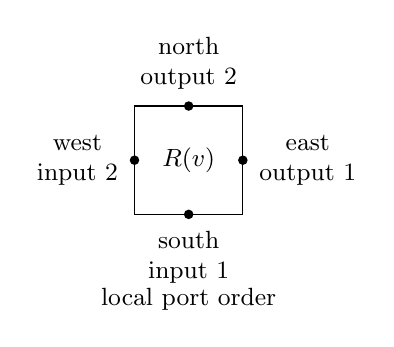
\begin{tikzpicture}[scale=.86,every node/.style={font=\small}]
 \draw (-.8,-.8) rectangle (.8,.8);
 \node at (0,0) {$R(v)$};
 \foreach \x/\y in {0/-.8,-.8/0,.8/0,0/.8}
    \fill (\x,\y) circle (2pt);
 \node[below,align=center] at (0,-.9) {south\\input 1};
 \node[left,align=center] at (-.9,0) {west\\input 2};
 \node[right,align=center] at (.9,0) {east\\output 1};
 \node[above,align=center] at (0,.9) {north\\output 2};
 \node at (0,-2.05) {local port order};
\end{tikzpicture}
\hspace{1cm}
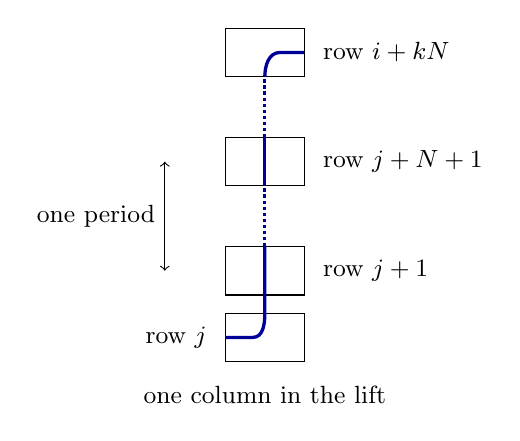
\begin{tikzpicture}[scale=.77,every node/.style={font=\small}]
 \foreach \y in {0,1.1,2.9,4.7}
    \draw (-.65,\y-.4) rectangle (.65,\y+.4);
 \draw[very thick,blue!60!black] (-.65,0) -- (-.2,0)
     to[out=0,in=-90] (0,.4) -- (0,1.5);
 \draw[very thick,blue!60!black,densely dotted] (0,1.5) -- (0,2.5);
 \draw[very thick,blue!60!black] (0,2.5) -- (0,3.3);
 \draw[very thick,blue!60!black,densely dotted] (0,3.3) -- (0,4.3);
 \draw[very thick,blue!60!black] (0,4.3)
     to[out=90,in=180] (.25,4.7) -- (.65,4.7);
 \node[left] at (-.8,0) {row $j$};
 \node[right] at (.8,1.1) {row $j+1$};
 \node[right] at (.8,2.9) {row $j+N+1$};
 \node[right] at (.8,4.7) {row $i+kN$};
 \draw[<->] (-1.65,1.1) -- (-1.65,2.9)
     node[midway,left] {one period};
 \node[below,align=center] at (0,-.65) {one column in the lift};
\end{tikzpicture}
\caption{The boxes show cyclic port order, rather than physical angles.
On the right, dotted portions contain the omitted intermediate rhombi.
The two displayed south--north passages are one period apart, so they
visit the same vertices after projection onto the cylinder. In the
planar lift all rhombi used are distinct.}
\label{fig:E-local-connector}
\end{figure}

Concatenate lifts of bridges counted by the divergent entry with
copies of this connector, always in successive disjoint column slabs.
Their interiors are disjoint, so the resulting planar path is
self-avoiding. To recover the concatenation, list all column cuts
that the path meets exactly once. Between two adjacent column cuts
in this list, a width-one subbridge inside any original valid slab
is still projection-valid. The inserted connectors are precisely the
projection-invalid width-one subbridges: they occupy one entire
column and their two cuts are crossed only at their endpoints.
Thus the connectors, the intervening slabs, and their original paths
are uniquely recovered from the concatenated path.

Choose finitely many valid slab widths whose total mass is $B$ with
$aB>1$. The width generating function of one valid-slab--connector
block is $g(z)=a\sum_M b_M(i,j)z^{M+1}$, with the sum restricted to
those widths. It satisfies $g(0)=0$ and $g(1)>1$. Hence the generating
function $\sum_{r\ge0}g(z)^r$ of recoverable concatenations has radius
strictly less than one. Each slab has at most a fixed constant times
its width in vertices, because its projection is self-avoiding on a
fixed cylinder; the connector has bounded length. Consequently all
these planar paths of total width $w$ have length at most $C_Nw$.
Their total critical weight is bounded above by the sum of
$c_n\rho^n$ for $n\le C_Nw$, up to fixed endpoint factors. This is
$\exp(o(w))$ by Proposition~\ref{prop:02-critical}, contradicting the
radius just obtained.

\end{proof}

\begin{proposition}[Physical cylinder vacuum]
At physical row parameters $u_i\in\{\lambda,2\lambda\}$,
\label{prop:02-cylinder-vacuum}
the column $T(3\lambda)$ restricted to vectors with zero empty
component has spectral radius less than one. Its unique stationary
state with empty component one is the regular continuation of $U_N$.
It equals the absolutely convergent sum of half-cylinder configurations
with vacant far boundary. The right-half state is
$U_N(3\lambda-u_1,\ldots,3\lambda-u_N)$.
\end{proposition}
\begin{proof}
A nonzero diagram propagated from a nonempty input pairing either
has a west-to-east spanning path or closes a discarded cycle. The
number of path segments is bounded at fixed $N$. Discarding their
mutual avoidance bounds their weights by a product of an exponentially
decaying spanning sum from Lemma~\ref{lem:02-periodic-slab} and
subexponential same-side sums. Therefore
the transfer on the subspace of zero empty component has spectral
radius strictly below one. The empty component itself is invariant.
Writing the transfer in these two blocks proves uniqueness and local
analyticity of its normalized fixed vector, and convergence from a
vacant far boundary proves the half-cylinder interpretation.
The rational stationary vector $V_N/h_N$ agrees with it wherever
defined nearby, hence extends to the physical parameters. Horizontal
reflection gives the stated right-half arguments. Vertical reflection
also recovers the covariance proved algebraically above.
\end{proof}

\subsection{The finite separating-loop formula}

Split the cyclic list into consecutive groups $X,Y$ of sizes $s,b$,
where $N=s+b$, and mark the two seams. Define $Z_{X,Y}(\chi)$ by
contracting the left and right vacuum states, assigning a closed loop
weight $\chi$ if it crosses the $X$ portion of the cut an odd number
of times, and weight zero otherwise. The empty configuration contributes
one. If a group is empty all loops have weight zero, so $Z=1$.
At physical parameters the markers are face centers. Compactifying
the cylinder ends gives a sphere, on which the odd-intersection rule
is precisely separation of the markers. Therefore $Z_{X,Y}(\chi)$
counts disjoint polygon families all separating the markers, with
weight $\prod_\ell\chi\rho^{|\ell|}$. Every such loop meets the cut;
disk connectivity on its two sides suffices to test separation.
The half-cylinder sums converge absolutely, and a family has a
bounded number of loops at fixed $N$, so this interpretation is valid
for every fixed $\chi$.

For the balanced observable $Z_N$ of the introduction, $N=2m$ and
the prescribed row list is $m$ copies of $2\lambda$ followed by $m$
copies of $\lambda$. Identify the triangular lattice with the complex
plane and start its column cut at the face center $f_1=0$. Its successive
edges have these row vectors, so the second marker and period are
\[
 f_2=m e^{2\pi i/3}=-\frac N4+i\frac{N\sqrt3}{4},\qquad
 V=m(e^{2\pi i/3}+e^{\pi i/3})=i\frac{N\sqrt3}{2}.
\]
The two groups are the two portions of this prescribed cut from $0$
to $f_2$ and from $f_2$ to $V$. Translation or reflection gives the
same observable. In particular the markers are half a period apart in
height; their longitudinal displacement is fixed by this construction.

\begin{lemma}[Characterization of the contraction]\label{lem:02-characterization}
The rational functions $Z_{X,Y}(\chi)$ are uniquely determined by the
following properties, with $\chi$ fixed.
\begin{enumerate}
\item $H_{X,Y}=h_N(X,Y)^2Z_{X,Y}$ is polynomial of degree at most
$2N-2$ in each argument, and $Z$ is symmetric within each group.
\item An ascending merge or deletion within either group leaves $Z$
unchanged after making the corresponding replacement or deletion.
\item Sending one argument to zero or infinity omits that site.
\item Sending $x\in X$ and $y\in Y$ to infinity at fixed generic
ratio gives
\[
 Z_{X,Y}\longrightarrow Z_{\widehat X,\widehat Y}Z_{x,y},
 \qquad Z_{x,y}=1+\chi(2c)^2\frac{xy}{(x+y)^2}.
\]
\item At size zero, $Z=1$.
\end{enumerate}
All limits are rational limits at generic values of the remaining
arguments. Hats mean omission of the indicated sites.
\end{lemma}
\begin{proof}
The right-half arguments are $q^3/x_i$. Equation~\eqref{eq:02-reciprocity},
homogeneity, and the per-slot degree bounds for $V_N$ give the
polynomial bound for $H$: occupied half-powers occur in pairs in the
contraction. To exchange sites within a group, move a symmetric braid
box from one side of the contraction to the other by transposition.
The two states braid in opposite directions because the starred
arguments reverse differences. Loop parity is preserved: following
the arcs in the box layer shows that each resulting loop has an even
total number of $X$-hits on the two interfaces of that layer. Thus
any cycle discarded on one side has zero gluing weight as well.
This proves symmetry and also permits a same-group splitting layer
to be moved through the contraction. At the descending specialization
on the starred side, apply $R(j\lambda)=S_jS_j^{\mathsf t}$ and the
ascending splitting identity. To cancel $S_j$, project its output onto diagrams whose first new
slot is vacant. For $S_2$, omitting that slot leaves the diagonal map
with coefficients $1$ on a vacancy and $\rho$ on an occupied strand.
For $S_3$, both new slots are then vacant; omitting them gives the
identity. Thus $S_j$ is injective, and
$S_jU_{\rm red}=S_jS_j^{\mathsf t}U_{\rm desc}$ implies
$S_j^{\mathsf t}U_{\rm desc}=U_{\rm red}$. This proves
the reduction of $Z$.

Cyclic covariance and the last-slot leading coefficient show that
sending one argument to infinity inserts a vacant site in the left
vacuum. Reflection gives the same statement in the right vacuum.
Horizontal reflection gives the limit at zero.

For completeness, the simultaneous two-site limit requires more than
the individual limits. Reorder within groups so that $x,y$ are adjacent
across a marker, and rotate them to the last two positions. Write
$P$ for the other $N-2$ arguments. We claim
\begin{equation}\label{eq:02-pair-limit}
 \frac{V_N(P,x,y)}{(xy)^{N-2}}
 =V_{N-2}(P)\otimes V_2(x,y)+o(|x|),
 \qquad
 V_2(x,y)=(x+y)\varnothing+2c\sqrt{xy}\,\mathrm{cup}.
\end{equation}
Fix square-root branches on the scaling ray. In the interpolation in
$y$, the deletion nodes are $y_z=q^3z$ for $z\in(P,x)$. For $N\ge3$,
nodes belonging to $P$ have data $O(|x|^{N-1})$, cardinal factors
$O(|x|^{N-3})$, and additional occupied square-root ratios at most
$O(|x|^{1/2})$. After division by $(xy)^{N-2}$ they are $o(|x|)$.
The leading vacant interpolation term becomes
$(y-y_x)V_{N-2}\otimes\varnothing+o(|x|)$. At $y_x=q^3x$ the data are
\[
 (x+y_x)\prod_{p\in P}(p-q^{-3}x)(p-q^6x)\,S_3V_{N-2}(P).
\]
The cardinal factor is asymptotic to $(y/y_x)^{N-2}$, with an extra
$\sqrt{y/y_x}$ on occupied output. Since $q^{-3}q^6=q^3$, these
terms give exactly the remaining terms in Equation~\eqref{eq:02-pair-limit}.
The expression for $V_2$ follows directly from the size-two
interpolation. Division by the empty components gives factorization
of the normalized left vacuum, and reflection gives that of the
right vacuum. The intersection-parity rule factors on the two
subsystems, proving both the pair limit and the displayed $Z_{x,y}$.

To prove uniqueness, the zero-site value and omission already settle
$N=1$. At $N=2$ with one site in each group, omission at zero and
infinity leaves only a possible difference $Cxy$ of the cleared
numerators. Its quotient by $h_2^2=(x+y)^2$ has a nonzero paired
scaling limit unless $C=0$, so the specified pair limit settles this
case. For all other group sizes, induct on $N$ and subtract two
candidate cleared polynomials. The known
scalar reductions of $h_N$ turn the reductions of $Z$ into identical
values of these polynomials at each split. Omission at zero kills
their constant coefficient, and
omission at infinity kills their leading coefficient. In a variable
of a group of size $s$, symmetry and the two reductions supply
$4(s-1)$ roots, namely $q^{\pm2}$ and $q^{\pm3}$ times every other
same-group argument. If $s>b$, these roots, together with the zero
constant coefficient, exceed the remaining degree $2N-3$.
If $s=b\ge2$, the difference must be a constant multiple of
\begin{equation}\label{eq:02-uniqueness-factor}
 \left(\prod_i x_i\right)
 \prod_{\substack{i<j\\\text{same group}}}
       (x_i^2+x_j^2)D_0(x_i,x_j).
\end{equation}
Indeed its degree in each variable is $1+4(s-1)=2N-3$, exactly the
remaining bound, so the quotient has degree zero in every variable.
When one argument from each group tends to infinity, this factor has
the same leading order as $h_N^2$ and a nonzero generic coefficient.
The pair limit forces the rational difference to tend to zero, so
its constant multiplier vanishes. The size-zero and size-two
conditions cover the remaining balanced cases.
\end{proof}

Using the fixed square roots, define the centered normalization
$\widetilde h_N=h_N\prod_i x_i^{-(N-1)/2}$. Its square is
\[
 \widetilde h_N^2=\frac{h_N^2}{\prod_{i<j}x_ix_j}
                 =\frac{h_N^2}{\prod_i x_i^{N-1}}.
\]
\paragraph{The three labels as formal site strings.}
Before writing the label sum, we construct its pair weights. Give a
site in group $\sigma=+1$ on $X$ or $\sigma=-1$ on $Y$ a generic
logarithmic coordinate $a_i$, with $x_i=e^{a_i}$. Here $a_i$ denotes
a logarithm, distinct from the earlier open-strip cosine coordinate.
Attach a formal string of length $a\in\{0,1,2\}$ at
\[
 a_i+i\sigma\beta,\ldots,a_i+i\sigma a\beta,
 \qquad l=\sigma(1-a).
\]
These are prescribed spectral points, with no integration variables
yet; at length zero the string is empty. Thus the three labels record
the three possible string lengths.
At this stage we assign weights only between distinct site strings;
factors within one string, which have poles at these spectral points,
will later be evaluated by residues.
We will first verify the resulting finite algebraic formula, and then
realize these strings as residues of a particle integral.

Put $P_j(r)=-2\sinh((r+ij\beta)/2)$. Products below are evaluated
at the coordinate difference of their arguments. For two objects
in the same group, the site--site, particle--site, and
particle--particle factors are, respectively,
\begin{equation}\label{eq:02-same-factors}
 B_s=P_2P_{-2}P_3P_{-3},\qquad
 F_s=(P_1P_{-1})^{-1},\qquad
 E_s=P_0^2P_2P_{-2}F_s.
\end{equation}
For different groups always use the plus coordinate minus the minus
coordinate, and use
\begin{equation}\label{eq:02-cross-factors}
 B_c=P_2^2P_3^2,\qquad F_c=P_1^{-2},\qquad E_c=P_0^2P_2^2F_c.
\end{equation}
The same-group factors are even, so no ordering convention is needed
there.

For ordered groups $\sigma,\omega$ and site labels $l,k$, let
$a=1-\sigma l$ and $b'=1-\omega k$, with the plus group first
when they differ. Let $z$ be the difference of the two site coordinates.
Multiply their site--site factor, all factors from a particle in either
string to the other site, and all factors between particles in different
strings. Denote this mutual product by
$\mathcal S^{\sigma\omega}_{lk}(z)=\prod_jP_j(z)^{n_j}$.
No factor internal to either string occurs. The exponents are encoded by
the Laurent polynomial
\begin{equation}\label{eq:02-string-polynomial}
 \sum_j n_j\xi^j=B-F(A+D)+EAD,\qquad
 A=\sum_{h=1}^a\xi^{\sigma h},\qquad
 D=\sum_{h=1}^{b'}\xi^{-\omega h}.
\end{equation}
Here, for $\sigma=\omega$,
\[
 B=\xi^2+\xi^{-2}+\xi^3+\xi^{-3},\quad F=\xi+\xi^{-1},\quad
 E=2+\xi^2+\xi^{-2}-F;
\]
for $\sigma=1,\omega=-1$,
\[
 B=2\xi^2+2\xi^3,\qquad F=2\xi,\qquad E=2+2\xi^2-F.
\]
Labels $l,r$ belong to $\{1,0,-1\}$, also denoted $+,0,-$, and
$v_l=2+l^2$. For a pair of sites set $e=1$ if they belong to the
same group and $e=-1$ otherwise. The arrays below are indexed by
$j\in\Z/8\Z$. A bracket $[a,b,\ldots]$ denotes the sum of the
corresponding unit vectors; repeated entries are counted with their
multiplicity. Rows and columns are ordered $+,0,-$; a matrix entry $0$ is the zero
vector, whereas an entry $[0]$ is the unit vector at residue zero:
\begin{equation}\label{eq:02-m-arrays}
\begin{split}
 m^+&=\begin{pmatrix}
 [2,3,5,6]&[3,5,6]-[0]&[5,6]-[0,1]\\
 [2,3,5]-[0]&[2,3,5,6]-[1,7]&[3,5,6]-[0]\\
 [2,3]-[0,7]&[2,3,5]-[0]&[2,3,5,6]
 \end{pmatrix},\\
 m^-&=2\begin{pmatrix}
 0 &[5]&[5,6]\\
 [3]&[4]&[5]\\
 [2,3]&[3]&0
 \end{pmatrix}.
\end{split}
\end{equation}
Define
\begin{equation}\label{eq:02-Q}
 Q^e_{lr}(u)=q^{ev_lr}u^{-1-elr}
       \prod_{j=0}^7(1-uq^{-j})^{m^e_{lr}[j]}.
\end{equation}

Substitution of $a,b'\in\{0,1,2\}$ gives
$\sum_{j\equiv-h\ (8)}n_j=m^{\sigma\omega}_{lk}[h]$.
Since
\[
 P_j(z)=e^{-(z+ij\beta)/2}(1-e^zq^j),
\]
the ratio of $Q^{\sigma\omega}_{lk}(e^z)$ to the string product is
$q^{\sigma\omega v_lk+\sum_j jn_j/2}$.
Differentiating Equation~\eqref{eq:02-string-polynomial} at $\xi=1$
gives the pair-phase identity
\begin{equation}\label{eq:02-string-phase}
 \frac{Q^{\sigma\omega}_{lk}(e^z)}{\mathcal S^{\sigma\omega}_{lk}(z)}
 =q^{\sigma\omega(v_lk+v_kl)/2}
 \begin{cases}
 1,&\sigma=\omega,\\
 (-1)^{1-lk},&\sigma=1,\ \omega=-1.
 \end{cases}
\end{equation}


\begin{theorem}[Finite cylinder formula]\label{thm:02-finite-formula}\label{E:finite-cylinder}
For $\chi=q^{-3}\tau+q^3\tau^{-1}$ and $\tau\ne0$,
\begin{equation}\label{eq:02-finite-formula}
 \widetilde h_N^2Z_{X,Y}(\chi)
 =\sum_{\substack{l_i\in\{-1,0,1\}\\
           \sum_{i\in X}l_i=\sum_{i\in Y}l_i=M}}
       \tau^M(-2c)^{\sum_i l_i^2}
       \prod_{i<j}Q^{e(i,j)}_{l_il_j}(x_i/x_j).
\end{equation}
The sum includes all allowed integers $M$. Apparent singularities at
colliding arguments are evaluated by continuation.
\end{theorem}
\begin{proof}
We verify the characterization in Lemma~\ref{lem:02-characterization}.
The arrays satisfy
\[
 \sum_jm^e_{lr}[j]=2+2elr,\qquad
 \sum_jj\,m^e_{lr}[j]\equiv e(v_lr-v_rl)\pmod8,
\]
and their exponents reverse under transposition. These identities give
$Q^e_{lr}(u)=Q^e_{rl}(1/u)$ and hence within-group symmetry.
The only possible finite nonzero poles are same-group poles at
$u=1,q,q^{-1}$. At $u=1$ only unequal labels are singular, with simple
poles, and exchanging these labels cancels the residues. At $u=q$
the singular labels are $(+,-)$ and $(0,0)$. The first kernel divided
by the second tends to $-1/(4c^2)$; the ratio of the corresponding
spectator products for a spectator of label $k$ and relative type
$e$ is $q^{ek}$. Neutrality makes the product of these spectator
ratios one. The site weight ratio is $4c^2$, so the residues cancel.
Reciprocity treats $q^{-1}$. Cross-group kernels have no such poles.

Here are the finite calculations that also verify the reductions.
For a same-group pair $x,y$, put $u=x/y$ and $w=qy$:
\[
\begin{array}{c|c|c}
 u&(l,r)&\text{nonzero value or pole coefficient}\\\hline
 q\ \text{(pole)} &(+,-),(0,0)&-i(2+2\sqrt2),\quad 2i\sqrt2\\
 q^2 &(+,0),(+,-),(0,-)&2q,\quad(2c^2)^{-1},\quad2q^{-1}\\
 q^3 &(+,-)&1
\end{array}
\]
In the first row the entries mean pole coefficients, obtained after
multiplication by $1-u/q$. At $q^2$, set
$L=l+r$ and $J=v_l+v_r-v_L-l+r$; the three surviving cases have
$J=1,2,1$. Their spectator ratios are
\[
 \frac{Q^e_{lk}(x/z)Q^e_{rk}(y/z)}{Q^e_{Lk}(w/z)}
       =q^{eJk}\frac{(w+z)^2}{wz}.
\]
At $q^3$ the product of spectator factors is
\[
 Q^e_{+k}(x/z)Q^e_{-k}(y/z)
 =q^{3ek}\frac{(z-q^{-3}y)^2(z-q^6y)^2}{xyz^2}.
\]
These identities require only the following identities of the
exponent arrays, with indices taken modulo eight:
\[
\begin{split}
 m^e_{+k}[j+1]+m^e_{-k}[j]
     &=m^e_{0k}[j+1]+m^e_{0k}[j],\\
 m^e_{lk}[j+1]+m^e_{rk}[j-1]-m^e_{Lk}[j]
     &=2\delta_{j,4}\qquad(u=q^2),\\
 m^e_{+k}[j+3]+m^e_{-k}[j]
     &=2\delta_{j,2}+2\delta_{j,3}\qquad(u=q^3).
\end{split}
\]
The constants follow from
$1-q^a=-2ie^{ia\beta/2}\sin(a\beta/2)$.
For the spectators, neutrality gives $\sum ek=-(l+r)$.
Including site weights, the $q^2$ reduction is therefore multiplication
by
\[
 2\prod_z\frac{(w+z)^2}{wz},
\]
and the $q^3$ reduction is multiplication by
\[
 (2c)^2\prod_z\frac{(z-q^{-3}y)^2(z-q^6y)^2}{xyz^2}.
\]
These are precisely the homogeneous scalar quotient rules for
$\widetilde h_N^2$; division verifies the two reductions of $Z$.

For a single argument $x$ with label $l$, reciprocity and neutrality
bound the product of its interactions by order $x^{N-1-l^2}$ at
infinity and $x^{-(N-1)+l^2}$ at zero. Only $l=0$ contributes at
leading order. Its phases multiply to one, leaving respectively
$\prod_zx/z$ and $\prod_zz/x$, exactly the leading factors of
$\widetilde h_N^2$. Pole cancellation and these bounds also prove
the required polynomial degree after removing the centering.

For $x\in X,y\in Y$ tending to infinity together, interactions with
the remaining arguments have order
$|x|^{2(N-2)-(l-r)^2}$. Only $l=r$ survives at leading order.
Neutrality cancels the phases and ratio powers, leaving
$\prod_zxy/z^2$ times the separate pair and remaining expressions.
This agrees with Equation~\eqref{eq:02-pair-limit} for the scalar
normalization. Finally, the two-site sum over the three equal labels
is
\[
 \frac{(x+y)^2}{xy}+\chi(2c)^2,
\]
and the zero-site sum is one. Lemma~\ref{lem:02-characterization}
now proves the formula.
\end{proof}

\subsection{Contour sectors and residue cancellation}

For the asymptotic application, $s=b=m$, $N=2m$, and the arguments
in $X,Y$ will be respectively $1,q^{-1}$. These are obtained from the
physical row parameters $2\lambda$ on $X$ and $\lambda$ on $Y$, whose
$x$-values are $q^2,q$, by the common rescaling $x_i\mapsto q^{-2}x_i$.
Homogeneity of $V_N$ and $h_N$ leaves their quotient and the contraction
unchanged. We first keep the two rays apart and allow distinct real
offsets. Denote the groups by
$\sigma=+1,-1$, in that order, and set
\[
 \alpha_+=0,\qquad \alpha_-=-\varepsilon\beta,\qquad
 0<\varepsilon<1.
\]
Specialize the logarithmic site coordinates to
$\Im a_i=\alpha_{\sigma_i}$. Eventually $\varepsilon=1$ and the real offsets coalesce to zero.

A particle of group $\sigma$ at shift $j$ has coordinate
$u+i\alpha_\sigma+i\sigma j\beta$, with $u\in\R$ and measure
$du/(2\pi)$. There are three species in each group:
\[
\begin{array}{c|c|c}
 \text{species}&\text{shifts of its elementary particles}&\text{activity}\\\hline
 \text{main singleton}&0&p_\sigma\\
 \text{far singleton}&11/4&-p_\sigma\\
 \text{far double}&5/2,\ 7/2&4c^2p_\sigma^2
\end{array}
\]
The signed far species make the residue representation exact. When the
main contours are moved outward, particles left on the far contour
cancel against the negative far singletons; a particle attaching to
one of those singletons cancels an original far double. The surviving
configurations will therefore be strings of zero, one, or two particles
attached to each site. The proof below establishes this cancellation
with the factorials and phases retained.

The two constituents of a double share one real variable. For fixed
numbers $n_\sigma,t_\sigma,D_\sigma$ of the three species, multiply
all site--site factors, all particle--site factors, and all
particle--particle factors between elementary constituents, omitting
the internal $E_s$ between the two constituents of a single double.
Integrate over the real variable of every singleton and double.
Multiply the integral by
\[
 \prod_{\sigma=\pm1}
 \frac{p_\sigma^{n_\sigma}(-p_\sigma)^{t_\sigma}
                   (4c^2p_\sigma^2)^{D_\sigma}}
      {n_\sigma!\,t_\sigma!\,D_\sigma!}.
\]
Let $I$ denote the sum of these terms through total elementary degree
$\sum_\sigma(n_\sigma+t_\sigma+2D_\sigma)\le N$. This finite
truncation is sufficient for every coefficient used below; no
convergence assertion for an infinite activity series is needed.

\begin{theorem}[Contour-sector representation]\label{thm:02-contour-sectors}\label{E:contour-sectors}
For the prescribed site rays, every $0<\varepsilon<1$, and every
$\eta\in\mathbb C$, put $\chi=2\cos\eta$. Then
\begin{equation}\label{eq:02-contour-sectors}
 \widetilde h_N^2Z_{X,Y}(2\cos\eta)
 =(2d)^N\sum_{M=-\min(s,b)}^{\min(s,b)}
       (-1)^{sb+M}e^{i\eta M}
       [p_+^{s-M}p_-^{b+M}]I.
\end{equation}
The coefficient integrals are absolutely convergent. The identity
extends to $\varepsilon=1$ and to coincident real site offsets by
continuation and dominated convergence of the fused integrands.
\end{theorem}
\begin{proof}
\emph{Integrability and contour geometry.}
All coefficient terms on the right have exactly $N$ elementary
particles, because $(s-M)+(b+M)=N$. A particle at real coordinate $u$ receives decay
$O(e^{-N|u|})$ from the $N$ sites; a pair interaction grows at most
$O(e^{|u-u'|})$. The inequality
$|u-u'|\le|u|+|u'|$ therefore bounds the full integrand away from
its prescribed poles by a constant times
$\exp(-\sum|u|)$, counting elementary coordinates with multiplicity.
The same estimate applies to smaller elementary degree and to
fused particles or residues. Constants may depend on $N$, sites,
and the fixed contours. This proves the convergence needed for
contour movements and removal of their vertical ends.

For $\varepsilon<1$, temporarily move the far singletons to a common
shift $h$ and the far doubles to $h-1,h$, where
\[
 3<h<\frac{7-\varepsilon}{2}.
\]
The offsets are measured outward from each group's site ray, in units
of $i\sigma\beta$:
\[
\begin{array}{c|c|c}
 &\text{fixed offsets}&\text{temporary offsets}\\\hline
 \text{main singleton}&0&0\ \longrightarrow\ h\\
 \text{far singleton}&11/4&h\\
 \text{far double}&(5/2,7/2)&(h-1,h)\\
 \text{site residues}&\text{none initially}&1\ \text{or}\ (1,2).
\end{array}
\]
A parenthesized pair shares one real coordinate. Only the far contours
are moved in this first step; the main-contour arrow is the subsequent
deformation. Moving the far contours crosses no pole. Indeed the interaction of a double with any
particle has no poles after its two constituents are multiplied.
Relative to the double midpoint, the same-group fused $E_sE_s$
has only positive exponents at shifts $\pm1/2,\pm5/2$; the cross-group
product has exponent two at $-1/2,5/2$. The same observation applies
to pairs of doubles. Far particle--site poles are avoided because
all far constituent shifts stay in $(2,7/2]$. For opposite-group
singletons the cross difference lies strictly between zero and seven
in shift units.

\emph{Residues and cancellation of unbound particles.}
Move the main contours from shift zero to shift $h$. A same-group
site can collect an ordered string of length $a=0,1,2$, at its own
coordinate plus $i\sigma\beta,\ldots,i\sigma a\beta$.
The first attachment occurs at shift one; interaction with it permits
a second at shift two. An attempted third at shift three is canceled
by the zero in its interaction with the first. Quadratic coincidence
zeros likewise cancel attempts to attach twice at the same root.
A main particle can also attach one unit below an original far
singleton, converting it into a double. These are all possibilities:
fused doubles have no particle poles, and $2h+\varepsilon<7$
excludes cross-group poles.

Here is an ordering of the deformation that avoids any ambiguity
from moving poles. Divide $[0,h]$ into generic layers of thickness
less than $1/3$, separating the levels $2$ and $h-1$. In each layer
move the remaining unbound variables one at a time; freeze every
picked residue immediately, including during the rest of that layer.
Unbound variables in a common group then never differ by a full unit
of shift, so they do not create poles with one another. For fixed
generic distinct real coordinates of original far particles, also
distinct from site offsets, these are ordinary one-variable contour
moves across simple poles. An attached far spectator appears as the
complete double interaction. An unconverted far singleton is more
than one shift unit beyond every site-bound root. Thus residual
integrands have no unaccounted coincident-spectator singularity and
satisfy the preceding decay bound. The identities can consequently
be integrated over the original far spectators as well.

The internal weight of a string, including its factors with its own
site and excluding activities, is
\begin{equation}\label{eq:02-string-residues}
 r_0=1,\qquad r_1=\frac1{2d},\qquad r_2=\frac{c^2}{d^2}.
\end{equation}
With measure $du/(2\pi)$, the oriented residue multiplier is
$i\sigma$. The first $F_s$ pole contributes $1/(2d)$. The second
attachment contributes $-4c^2$ from the $E_s$ pole at relative
$i\sigma\beta$, and $F_s(2i\sigma\beta)=-1/(2d)$ from its
site factor. Multiplication gives $r_2$. Attachment at relative
$-i\sigma\beta$, below a far singleton, instead contributes
$4c^2$.

Fix a site-string pattern. The effective far singleton activity is
$-p_\sigma+p_\sigma=0$, from original and unpicked main singletons.
The effective far double activity is
$4c^2p_\sigma^2+4c^2(-p_\sigma)p_\sigma=0$, from original doubles
and attached original singletons. These cancellations respect all
factorials. Explicitly, start in one group with $n,t,D$ particles of
the three species. If $r$ main particles fill the specified site
strings and $a$ attach to $a$ of the original far targets, summing
labeled assignments leaves factorial coefficient
\[
 \frac1{(n-r-a)!\,(t-a)!\,a!\,D!}.
\]
Each assignment determines exactly one contour term through its
choices at shifts $1,2,h-1$. The remaining two kinds of singleton
and two kinds of double can therefore be combined by the binomial
formula. This argument is coefficientwise in $p_+,p_-$, so all
canceling terms have the same elementary total. Only completely
site-bound configurations survive. In particular every cancellation
used for the degree-$N$ coefficients takes place inside the finite
truncation defining $I$.

\emph{Identification with the finite label formula.}
Assign label $l=\sigma(1-a)$ to a site in group $\sigma$ with string
length $a$. The coefficient constraints become
$\sum_{X}l_i=\sum_{Y}l_i=M$. We check their mutual weights explicitly.
Use the formal string weights and their pair-phase identity
\eqref{eq:02-string-phase} established before the finite formula.
To multiply these phases without a size restriction, put
$\sigma_i=1$ on $X$, $\sigma_i=-1$ on $Y$, and $v_i=2+l_i^2$.
Neutrality gives $\sum_i\sigma_i l_i=0$, while $l_i^3=l_i$. Hence
\[
\begin{aligned}
\frac12\sum_{i<j}\sigma_i\sigma_j(v_i l_j+v_j l_i)
 &=\frac12\left[
    \left(\sum_i\sigma_i v_i\right)
    \left(\sum_i\sigma_i l_i\right)-\sum_i v_i l_i\right]\\
 &=-\frac32\sum_i l_i=-3M.
\end{aligned}
\]
The cross sign is
$(-1)^{sb-(\sum_Xl_i)(\sum_Yl_i)}=(-1)^{sb-M^2}=(-1)^{sb+M}$.
Thus the product of all pair phases is exactly
$q^{-3M}(-1)^{sb+M}$. Finally, since $\sum_i a_i^{\mathrm{len}}=N$
for the string lengths $a_i^{\mathrm{len}}$,
\[
 (2d)^N\prod_i r_{a_i^{\mathrm{len}}}=(-2c)^{\sum_i l_i^2}.
\]
Indeed the per-site ratio of the right-hand weight to
$(2d)^a r_a$ is $(-2c)^{1-a}$, whose product is one.
Taking $\tau=q^3e^{i\eta}$ in Theorem~\ref{thm:02-finite-formula}
now proves Equation~\eqref{eq:02-contour-sectors}.

\emph{Confluent physical limits.}
Return the far contours to the fixed shifts in the definition of
$I$. Their fused pair products have no pole at $\varepsilon=1$.
On these fixed contours the same decay bound persists in a
neighborhood of that value and of confluent real site offsets.
This justifies both final limits.
\end{proof}

\begin{lemma}[Signs at the confluent rays]\label{lem:02-sector-signs}
At $\varepsilon=1$ with confluent real site offsets, extract constant
signs from the site factors and from each full pair of integration
variables, multiplying double constituents before doing so, so that
the value at zero real difference is positive, or its leading
quadratic coefficient is positive when it vanishes. Their logarithms
then satisfy conjugation under $u\mapsto-u$. They are regular on
$\R$ except for same-species coincidences with singular part
$2\log|u-u'|$, including double--double coincidences.
At fixed far counts, multiply the extracted signs by the explicit
prefactor $(-1)^{sb+M}$ in Equation~\eqref{eq:02-contour-sectors}.
The resulting sign has $M$-dependence exactly $(-1)^{fM}$, up to an
$M$-independent sign, where $f=f_X+f_Y$ is the number of far elementary
particles. The remaining explicit phase is $e^{i\eta M}$.
\end{lemma}
\begin{proof}
For real $r$, $P_j(-r)=-\overline{P_j(r)}$. Each fused product has
even total exponent, which gives the asserted conjugation after a
real sign has been extracted. Real zeros of an elementary factor occur
only at $r=0$ and $j\in8\mathbb Z$. Combine the exponents before
testing for a zero, in particular for the two constituents of a
double. Ordered by main singleton, far singleton, and far double,
the extracted pair signs and vanishing orders are
\[
\begin{array}{c|c|c}
 &\text{sign matrix}&\text{order matrix at }r=0\\\hline\noalign{\vskip 3pt}
\text{same group}&
 \begin{pmatrix}+&-&+\\-&+&+\\+&+&+\end{pmatrix}&2I_3\\\noalign{\vskip 3pt}
\text{different groups}&
 \begin{pmatrix}-&-&+\\-&-&+\\+&+&+\end{pmatrix}&0.
\end{array}
\]
The site--particle signs are $(+,-,+)$ in the same group and
$(-,-,+)$ in different groups, with zero vanishing order in both
cases. These tables follow directly from $P_j(0)=-2i\sin(j\beta/2)$
and $P_{8k}(r)=-(-1)^kr+O(r^3)$: shift the exponents of
$P_0^2P_2P_{-2}/(P_1P_{-1})$ or $P_0^2P_2^2/P_1^2$ by every
constituent difference, add them, and cancel opposite powers. Thus
there are no other real singularities.

Let $n_\sigma,t_\sigma,D_\sigma$ count main singletons, far
singletons, and far doubles. Their elementary totals are
$K_+=s-M$ and $K_-=b+M$, with
$K_\sigma=n_\sigma+t_\sigma+2D_\sigma$.
The cross-group site and pair signs in the table have parity
\[
 bK_++sK_-+K_+K_-\equiv sb+M\pmod2.
\]
This cancels the prefactor in Equation~\eqref{eq:02-contour-sectors}.
The remaining negative factors are a same-group main--far-single
pair, a same-group far-single--site pair, and each far-single activity.
Their total parity is
\[
 (n_++s+1)t_++(n_-+b+1)t_-
 \equiv M(t_++t_-)\equiv Mf\pmod2,
\]
because $t_\sigma^2\equiv t_\sigma$ and
$f=t_++t_-+2D_++2D_-$. Doubles contribute only positive signs in
the tables. Any fixed extraction of the site--site signs is independent
of $M$. This proves the required imbalance phase.
\end{proof}

\subsection{The Pfaffian denominator at confluence}

The reference-kernel reduction uses Schur's Pfaffian identity and
Cauchy's determinant identity; see
\cite[equations (1.1)--(1.2)]{IshikawaOkadaTagawaZeng2006}.
We include their elementary forms in the present normalization.
The confluent kernel and its determinant asymptotic then require
the operator estimates below. This is an estimate for equal group
sizes. The contour identity above holds for unequal sizes as well,
but the present denominator theorem does not assert an asymptotic
uniform in that larger parameter domain.

In this subsection $N=2m$, the first $m$ logarithmic sites are zero,
and the last $m$ are $-i\beta$, all understood as confluent limits.
Set
\[
 \gamma=\frac43=\frac\pi{3\beta},\qquad
 L=\frac{\log N}{\gamma},\qquad
 H_*(u)=\frac{e^{2u}+2de^u+1}{(e^u-1)e^{u/2}}
                       \tanh\frac{\gamma u}{2}.
\]
At $u=0$ use the removable continuation of $H_*$.

\begin{theorem}[Balanced denominator asymptotic]\label{thm:02-denominator}\label{E:balanced-denominator}
For $N=2m\ge2$, with exactly $m$ sites at each of $0,-i\beta$, the
normalization $h_N$ is nonzero. As $N\to\infty$ through these even
sizes,
\begin{equation}\label{eq:02-denominator}
 \log\left|
 \frac{\widetilde h_N^2}
      {(\gamma/2)^N\prod_{i<j}H_*(a_i-a_j)^2}
 \right|
 =\frac5{24}\log N+o(\log N).
\end{equation}
\end{theorem}
\begin{proof}
First take distinct sites. Write
\[
 K(u)=\frac{\sinh u}{\cosh u+d},\qquad
 K_0(u)=\tanh\frac{\gamma u}{2}.
\]
Equation~\eqref{eq:02-h-pfaffian} and the definition of $H_*$ give
\begin{equation}\label{eq:02-determinant-ratio}
 \frac{\widetilde h_N^2}{\prod_{i<j}H_*(a_i-a_j)^2}
 =\frac{\det[K(a_i-a_j)]}{\det[K_0(a_i-a_j)]}.
\end{equation}
Here we used the Pfaffian identity
\[
 \operatorname{Pf}\left[\frac{v_i-v_j}{v_i+v_j}\right]
       =\prod_{i<j}\frac{v_i-v_j}{v_i+v_j},\qquad v_i=e^{\gamma a_i}.
\]
To prove it, clear denominators: the numerator is an alternating
polynomial of Vandermonde degree and is therefore a constant times
the Vandermonde. The residue at $v_{N-1}=-v_N$, followed by induction
from size two, determines the constant to be one.

For an even-dimensional skew matrix $A$, adding the all-ones matrix
does not change its determinant. Indeed the rank-one determinant
formula gives the extra term $\boldsymbol1^{\mathsf t}
\operatorname{adj}(A)\boldsymbol1$, which is zero since
$\operatorname{adj}(A)$ is skew. Apply this to both matrices in
Equation~\eqref{eq:02-determinant-ratio}, then conjugate by the
diagonal factors $e^{-\gamma a_i/2}$. The resulting reference kernel
is
\[
 G_0(u)=e^{-\gamma u/2}(1+K_0(u))
       =\operatorname{sech}(\gamma u/2),
\]
and the actual kernel is $G(u)=e^{-\gamma u/2}(1+K(u))$.
With Fourier convention $\widehat f(k)=\int_\R e^{-iku}f(u)\,du$
and $\zeta=\gamma/2+ik$, their transform ratio is
\begin{equation}\label{eq:02-fourier-ratio}
 \frac{\widehat G(k)}{\widehat G_0(k)}
 =\gamma\frac{\cos(\beta\zeta)\sin(\pi\zeta/\gamma)}
                    {\sin(\pi\zeta)}
 =\frac\gamma2(1+R(k)),\qquad
 R(k)=\frac1{2\cos(2\beta\zeta)}.
\end{equation}
For the first equality, put $t=e^u$ and use
\[
 1+K(u)=\frac{t}{t+e^{i\beta}}+\frac{t}{t+e^{-i\beta}},\qquad
 \int_0^\infty\frac{t^{p-1}}{1+t}\,dt=\frac\pi{\sin\pi p}.
\]
The beta integral follows by a keyhole contour, initially for
$0<\Re p<1$. The second equality in
Equation~\eqref{eq:02-fourier-ratio} follows from
$\pi/\gamma=3\beta$ and $\pi=4\beta$ by the triple-angle identity.

The determinant ratio is now explicit, but direct differentiation at
coalescing sites would obscure its size. We instead view the reference
matrix as a Gram matrix. Its orthogonal projection will occupy an
interval of length $2\gamma^{-1}\log N$ in the real direction; the
trace density on that interval will give the required logarithmic term.

We turn the determinant ratio into a finite-dimensional compression.
Let $\mathcal H$ be the Hilbert space with norm
\[
 \|f\|_{\mathcal H}^2
 =\int_\R|\widehat f(k)|^2v(k)\,\frac{dk}{2\pi},\qquad
 v(k)=\frac1{\widehat G_0(k)}
      =\frac\gamma{2\pi}\cosh\frac{\pi k}{\gamma}.
\]
Its functions have bounded evaluation at every
$z$ with $|\Im z|<\pi/(2\gamma)$. Write $k_z$ for the evaluation
vector, and $P=P_N$ for the orthogonal projection onto the span of
evaluations and their derivatives of orders $0,\ldots,m-1$ at
$z=\pm i\beta/2$. Centering the two site rays changes no differences. The derivative
evaluation vectors are linearly independent. Indeed, a linear relation
among them, written in Fourier variables and multiplied by the common
nonzero weight, has the form
$p_+(k)e^{\beta k/2}+p_-(k)e^{-\beta k/2}=0$ on $\mathbb R$, where
$p_+,p_-$ have degree at most $m-1$. Sending $k$ to $+\infty$ gives
$p_+=0$, and then $p_-=0$. Their Gram matrix is consequently positive
definite.

Start with distinct paired real offsets and permute columns by complex
conjugation; the reference matrix becomes the Gram matrix of these
evaluation vectors. The actual matrix represents the sesquilinear form with the
Fourier multiplier $\frac\gamma2(I+R)$ inserted. Passing to divided
differences gives the derivative vectors at confluence. Hence
\begin{equation}\label{eq:02-compression-determinant}
 \frac{\widetilde h_N^2}
 {(\gamma/2)^N\prod_{i<j}H_*(a_i-a_j)^2}
 =\det\left(I+PRP\big|_{\operatorname{ran}P}\right).
\end{equation}
The same column permutation is used in numerator and denominator,
so it introduces no sign in their ratio. The reference Gram matrix is
nondegenerate by the preceding independence argument.
Moreover $\operatorname{Re}R(k)\ge0$ for real $k$: since
$2\beta\operatorname{Re}\zeta=\pi/3$, the real part of
$\cos(2\beta\zeta)$ is $\tfrac12\cosh(2\beta k)>0$.
Thus $I+PRP$ is strictly accretive and invertible. Since the removable
factors $H_*(0)$ and $H_*(i\beta)$ are nonzero, the compression identity
already proves $h_N\ne0$ at these balanced confluent sites. The rest
of the proof determines its logarithmic size.

The projection has a useful exact localization formula:
\begin{equation}\label{eq:02-projection-complement}
 \|(I-P)k_z\|^2=\|k_z\|^2
 \prod_{\pm}
 \left|\frac{e^{\gamma z}-e^{\pm i\gamma\beta/2}}
 {e^{\gamma z}+\overline{e^{\pm i\gamma\beta/2}}}\right|^{2m}.
\end{equation}
To see this, augment the reference Gram matrix by $k_z$ and take its
Schur complement. Under $w=e^{\gamma z}$, its kernel is
$1/(w+\overline{w'})$ up to separate one-point factors. The Cauchy
determinant formula follows by clearing denominators and using
antisymmetry, with the constant fixed by residues. Its ratio after
augmentation is exactly Equation~\eqref{eq:02-projection-complement}.
Divided differences give its confluent version and prove the
nondegeneracy of the derivative Gram matrix.

For each fixed horizontal line in the evaluation strip, this implies
\begin{equation}\label{eq:02-projection-bound}
 \|Pk_z\|^2\le C\min\{1,Ne^{-\gamma|\Re z|}\}.
\end{equation}
Indeed, for $a=e^{\pm i\gamma\beta/2}$ and $w=e^{\gamma z}$,
\[
 1-\frac{|w-a|^2}{|w+\overline a|^2}
 =\frac{4\Re w\Re a}{|w+\overline a|^2}
 \asymp e^{-\gamma|\Re z|}.
\]
The product in Equation~\eqref{eq:02-projection-complement} is
therefore within $CNe^{-\gamma|\Re z|}$ of one, and is at most
$\exp(-cNe^{-\gamma|\Re z|})$. In particular, translated to the
frame of any real $x$ with $|x|\le(1-\delta)L$, the projections
$P_N$ converge strongly to the identity, uniformly for fixed
$\delta>0$. The complement tends uniformly to zero on every fixed
evaluation vector, and these vectors span a dense subspace by Fourier
uniqueness; contraction of the projections extends this to all of
$\mathcal H$.

Integrating Equation~\eqref{eq:02-projection-bound} on horizontal
lines near the two edges of the evaluation strip gives, for every
fixed $\epsilon>0$,
\begin{equation}\label{eq:02-trace-envelope}
 \operatorname{Tr}(Pe^{-\epsilon|k|}P)\le C_\epsilon L.
\end{equation}
Here multipliers are written as functions of $k$. More explicitly,
Plancherel on the line of height $y$ gives the multiplier
$v^{-1}e^{-2ky}$, and its trace against $P$ is
$\int_\R\|Pk_{x+iy}\|^2\,dx$. Choose $y$ near each strip edge.
The sum of the two resulting positive multipliers dominates a
constant multiple of $e^{-\epsilon|k|}$, while each integral is
$O(L)$ by Equation~\eqref{eq:02-projection-bound}.

We claim, for each integer $p\ge1$,
\begin{equation}\label{eq:02-trace-limit}
 \lim_{N\to\infty}\frac{\operatorname{Tr}((PRP)^p)}{2L}
       =\int_\R R(k)^p\,\frac{dk}{2\pi}.
\end{equation}
First truncate the exponentially decaying multiplier $R$ to a bounded
frequency interval. For any multiplier $H$,
\[
 \|PHP\|_1\le\operatorname{Tr}(P|H|P),
\]
by factoring through $|H|^{1/2}P$ and using the Hilbert--Schmidt
inequality. Equation~\eqref{eq:02-trace-envelope} makes the normalized
trace error tend to zero uniformly as the frequency interval grows;
a telescoping product gives the same statement for each fixed power.

For a bounded compactly supported symbol $S$, cyclicity of the trace
writes the corresponding trace as
\[
 \operatorname{Tr}\bigl(v^{-1}(Sv)P(SP)^{p-1}\bigr).
\]
The resolution
$\int_\R|k_x\rangle\langle k_x|\,dx=v^{-1}$ turns this trace into
$\int_\R F_N(x)\,dx$, where
\[
 F_N(x)=\left\langle(Sv)P(SP)^{p-1}k_x,k_x\right\rangle_{\mathcal H}.
\]
The real-line evaluation vectors have a fixed norm. The multiplier
$Sv$ is bounded on the compact frequency support, and the rightmost
operator acting on $k_x$ contains $P$. Hence
$|F_N(x)|\le C\|Pk_x\|$.
Translate $k_x$ to $k_0$ and conjugate every $P$ by the same real
translation. The multipliers are unchanged. In the bulk
$|x|\le(1-\delta)L$, strong convergence of these translated
projections therefore gives, uniformly,
\[
 F_N(x)\longrightarrow
 \left\langle S^pv k_0,k_0\right\rangle_{\mathcal H}
 =\int_\R S(k)^p\,\frac{dk}{2\pi}.
\]
The transition region has length $O(\delta L)$; beyond $(1+\delta)L$,
Equation~\eqref{eq:02-projection-bound} has an integrable exponential
tail of size $o(L)$. Divide by $2L$, then let $\delta\downarrow0$.
This proves the compact-frequency limit and hence
Equation~\eqref{eq:02-trace-limit}.

On the real frequency axis, $|R(k)|\le1$ and $\Re R(k)\ge0$:
here $2\beta\Re\zeta=\pi/3$. Moreover
$\|PRP\|_1=O(L)$ by Equation~\eqref{eq:02-trace-envelope}.
For $0<t<1$, the logarithmic power series and
Equation~\eqref{eq:02-trace-limit} yield
\[
 \lim_{N\to\infty}\frac1{2L}
       \operatorname{Tr}\log(I+tPRP)
 =\int_\R\log(1+tR(k))\,\frac{dk}{2\pi}.
\]
Accretivity gives $\|(I+tPRP)^{-1}\|\le1$ for $t\ge0$, so the
trace derivative is bounded by $\|PRP\|_1=O(L)$. The same integrable
bound holds for the limiting integral. Thus the limit extends to
$t=1$. Taking real parts is equivalent to taking the logarithm of
the determinant modulus in Equation~\eqref{eq:02-compression-determinant}.

Finally shift the contour from $\Re\zeta=\gamma/2$ to
$\Re\zeta=0$. The function
$\log(1+1/(2\cos(2\beta\zeta)))$ is analytic in the intervening
strip, with the branch tending to zero at imaginary infinity;
its horizontal-end contributions vanish exponentially. Therefore
\[
 \int_\R\log(1+R(k))\,dk
 =\int_\R\log\left(1+\frac1{2\cosh(2\beta k)}\right)\,dk
 =\frac{5\pi^2}{72\beta}.
\]
For the last evaluation use evenness and set $y=e^{-2\beta k}$ for
$k>0$. The logarithm becomes
$\log[(1-y^3)/((1-y)(1+y^2))]$. Termwise integration of its
convergent logarithmic series, or monotone limits of their integrals,
gives
\[
 \frac1\beta\int_0^1
 \frac{\log(1-y^3)-\log(1-y)-\log(1+y^2)}{y}\,dy
 =\frac1\beta\left(-\frac{\pi^2}{18}
                         +\frac{\pi^2}{6}-\frac{\pi^2}{24}\right)
 =\frac{5\pi^2}{72\beta}.
\]
Combining this with $2L/(2\pi)$ and
$\beta\gamma=\pi/3$ gives the coefficient
$5\pi/(72\beta\gamma)=5/24$ in
Equation~\eqref{eq:02-denominator}.
\end{proof}
